\documentclass[a4paper,english]{scrreprt}

% Uncomment to optimize for double-sided printing.
% \KOMAoptions{twoside}

% Set binding correction manually, if known.
% \KOMAoptions{BCOR=2cm}

% Localization options
\usepackage[german]{babel}
\usepackage[T1]{fontenc}
\usepackage[utf8]{inputenc}

% Enhanced verbatim sections. We're mainly interested in
% \verbatiminput though.
\usepackage{verbatim}

% PDF-compatible landscape mode.
% Makes PDF viewers show the page rotated by 90°.
\usepackage{pdflscape}

% Advanced tables
\usepackage{tabu}
\usepackage{longtable}
\usepackage{dcolumn}
\newcolumntype{d}[1]{D{.}{\cdot}{#1} }

% Fancy tablerules
\usepackage{booktabs}

% Graphics
\usepackage{graphicx}

% Current time
\usepackage[useregional=numeric]{datetime2}

% Float barriers.
% Automatically add a FloatBarrier to each \section
\usepackage[section]{placeins}

% Custom header and footer
\usepackage{fancyhdr}

\usepackage{geometry}
\usepackage{layout}

% Math tools
\usepackage{mathtools}
% Math symbols
\usepackage{amsmath,amsfonts,amssymb}
\usepackage{amsthm}

% SI units
\usepackage{siunitx}
\DeclareSIUnit\Molar{\textsc{m}}
\DeclareSIUnit\mole{mol}
\DeclareSIUnit\rpm{rpm}
\DeclareSIUnit\cfu{cfu}

% Chemistry
\usepackage{mhchem}

% Subfigures & captions
\usepackage{subcaption}
\usepackage{wrapfig}

\DeclarePairedDelimiter\abs{\lvert}{\rvert}

\pagestyle{plain}
% \fancyhf{}
% \lhead{}
% \lfoot{}
% \rfoot{}
% 
% Source code & highlighting
\usepackage{listings}

% Convenience commands
\newcommand{\mailsubject}{2027 - Lab course biochemistry 1}
\newcommand{\maillink}[1]{\href{mailto:#1?subject=\mailsubject}
                               {#1}}

% Should use this command wherever the print date is mentioned.
\newcommand{\printdate}{\today}

\subject{2027 - Lab course biochemistry 1}
\title{10 - Transformation des Darmbakteriums Escherichia Coli}

\author{Michael Senn \maillink{michael.senn@students.unibe.ch} - 16-126-880 - Gruppe 14}

\date{\printdate}

% Needs to be the last command in the preamble, for one reason or
% another. 
\usepackage{hyperref}


\begin{document}
\maketitle

\chapter{Einfürung}

\section{Zielsetzung}

Ziel des Experimentes war es, ein Plasmid in Bakterienzellen einzuschleusen,
und die Expression eines Fremdproteins zu untersuchen.

Hierzu wurde ein pGLO Plasmid - das unter anderem das Fluroeszenzprotein GFP,
und das Beta-Lactamase Enzym zwecks Antibiotika-resistenz codiert - in E. coli
Zellen eingeschleust, und deren Wachstum und Aussehen unter UV Licht auf
Nährmedium mit verschiedenen Zusatzstoffen untersucht.

\chapter{Durchführung\cite{skriptv10}}

\section{Steriles Arbeiten}

Wo immer nötig, wurde steril gearbeitet. Dies beinhaltete die Arbeit bei
offener Flamme eines Gasbrenners zwecks wegtragen von Keimen vom
Arbeitsobjeckt, und das steriliseren von Flaschenhälsen vor und nach Entnahme
von Stoffen.

\section{Herstellung und Sterilisation von Nährmedien und Materialien}

\SI{400}{\ml} LB Flüssigmedium (Luria-Broth) wurden in einem Becherglas
hergestellt. Hierzu wurden abgewogen:

\begin{itemize}
	\item \SI{4}{\g} Bacto tryptone
	\item \SI{2.29}{\g} Yeast extract
	\item \SI{4}{\g} \ce{NaCl}
\end{itemize}

\SI{400}{\ml} deionisiertes Wasser wurden abgewogen und vorsichtig dazugegeben.
Die Mischung wurde mit einem Magnetrürer aufgelöst.

In zwei \SI{150}{\ml} Duranflaschen wurden je \SI{2.25}{\g} Agar eingewogen,
und \SI{100}{\ml} LB Medium dazugegeben. Der Deckel wurde lose
daraufgeschraubt.

Der Rest des LB Mediums wurde in zwei \SI{50}{\ml} Flaschen gegeben, und alle
vier Flaschen autoklaviert.

Ein \SI{100}{\ml} Erlenmeyerkolben, und eine Büchse Glasauslaufpipetten wurde
vorgängig ebenfalls in der Autoklave sterilisiert.

\section{Platten giessen}

Nach dem Autoklavieren wurde der LB Nähragar in der Autoklave auf
\SI{60}{\celsius} abgekühlt. Im Anschluss wurden durch die zwei Gruppen drei
Flaschen vorbereitet - eine ohne Zugabe weiterer Stoffe, eine mit \SI{150}{\ul}
Ampizilin (Endkonzentration \SI{100}{\ug \per \ml}), und eine mit Ampizilin
(Endkonzentration \SI{100}{\ug \per \ml}) und Arabinose (Endkonzentration
\SI{1}{\milli\Molar}).

Petriplatten wurden beschriftet, und die hergestellten Lösungen auf je
mindestens 9 Platten verteilt. Die Platten wurden bei Raumtemperatur
ausgekühlt.

\section{Transformation von E. coli}

\subsection{Vorkultur}

Durch den Assistenten wurden zwei Vorkulturen angesetzt. \SIrange{2}{3}{\ml}
steriles LB Medium wurden je in zwei sterile Reagenzröhrchen gegeben. Eine
einzelne Kolonie der Agarplatten wurde in das Medium übertragen, und die
Kulturen bei \SI{37}{\celsius} über nacht in einem Rotationsschüttler
inkubiert.

\subsection{Hauptkultur}

\SI{0.9}{\ml} der am Vortag angesetzten Vorkultur wurden mit \SI{30}{\ml} LB
Medium in den sterilen Erlenmeyerkolben gegeben. Die Kultur wurde bei
\SI{37}{\celsius} auf dem Orbitalschüttler inkubiert, wobei alle \SI{30}{\min}
mit einer sterilen Pipette \SI{1}{\ml} entnommen wurde, um die optische Dichte
bei \SI{550}{\nm} zu bestimmen, wie in Tabelle \ref{tbl:od_kultur} und
Abbildung \ref{fig:od_kultur} dargestellt.

Bei Erreichen eines Wertes von 0.343 wurde die Kultur aus dem Schüttler
genommen und auf Eis abgekühlt.

\subsubsection{OD Werte während Inkubation}

\begin{table}
	\centering
	\begin{tabu}{ll}
		\toprule
		Inkubationszeit & Optische Dichte \\
		\midrule
		\SI{0}{\min} & 0.062 \\
		\SI{20}{\min} & 0.063 \\
		\SI{40}{\min} & 0.087 \\
		\SI{60}{\min} & 0.117 \\
		\SI{80}{\min} & 0.170 \\
		\SI{100}{\min} & 0.263 \\
		\SI{120}{\min} & 0.343 \\
		\bottomrule
	\end{tabu}
	\caption{OD Messung der Bakterienkultur bei \SI{550}{\nm} über Zeit}
	\label{tbl:od_kultur}
\end{table}

\begin{figure}[h]
	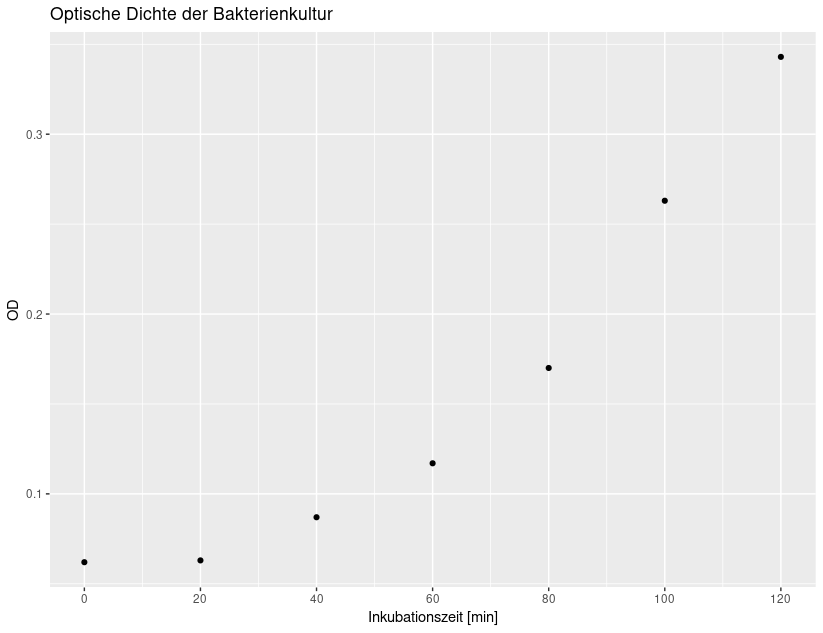
\includegraphics[width=0.9\textwidth]{img/od_kultur.png}
	\caption{OD Messung der Bakterienkultur bei \SI{550}{\nm} über Zeit}
	\label{fig:od_kultur}
\end{figure}

\subsection{Herstellen der kompetenten Zellen}
\label{sec:kompetente_zellen}

Die gekühlte Kultur wurde in ein vorgekühltes steriles \SI{50}{\ml}
Zentrifugenröhrchen gegossen. Die Röhrchen der beiden Gruppe wurden bei
\SI{4}{\celsius} im SS34 Rotor bei \SI{5000}{rpm} während \SI{10}{\min}
zentrifugiert.

Der Überstand wurde abgegeossen, und das Zellsediment in \SI{5}{\ml}
\SI{100}{\milli\Molar} \ce{CaCl2}-Lösung resuspendiert. Es wurde erneut unter
gleichen Bedingungen zentrifugiert, der Überstand abgegossen und in \SI{1}{\ml}
\SI{100}{\milli\Molar} \ce{CaCl2}-Lösung resuspendiert. Die Suspension wurde in
ein steriles vorgekühltes Eppendorfröhrchen transferiert und für circa eine
Stunde auf Eis gelassen. Hierraus wurden zwei Eppendorfröhrchen gemäss Tabelle
\ref{tbl:kompetente_zellen} hergestellt.

\begin{table}
	\centering
	\begin{tabu}{lll}
		\toprule
		& E1 & E2 \\
		\midrule
		Plasmid pGLO \SI{104.5}{\ng\per\ul} & \SI{2}{\ul} (\SI{209}{\ng} DNA) & - \\
		kompetente Zellen & \SI{0.2}{\ml} & \SI{0.2}{\ml} \\
		\midrule
		& \multicolumn{2}{l}{\SI{30}{\min} auf Eis stehen gelassen} \\
		& \multicolumn{2}{l}{Hitzeschock \SI{45}{\s} in \SI{42}{\celsius} Wasserbad} \\
		\midrule
		LB Medium & \SI{1}{\ml} & \SI{1}{\ml} \\
		\midrule
		& \multicolumn{2}{l}{\SI{30}{\min} bei \SI{37}{\celsius} im Brutkasten inkubiert} \\
		\bottomrule
	\end{tabu}
	\caption{Vorbereitung der kompetenten Zellen und der Negativkontrolle}
	\label{tbl:kompetente_zellen}
\end{table}

Im Anschluss wurde die transformierte und nicht transformierte Kontrolle wie in
Tabelle \ref{tbl:ausplattierung} ausplattiert.

\begin{table}
	\centering
	\begin{tabu}{lllllll}
		\toprule
		& \multicolumn{2}{c}{LB Platten} & \multicolumn{2}{c}{LB Amp Platten} & \multicolumn{2}{c}{LB Amp Ara Platten} \\
		\midrule
		E1 & \SI{10}{\ul} & \SI{100}{\ul} & \SI{10}{\ul} & \SI{100}{\ul} & \SI{10}{\ul} & \SI{100}{\ul} \\
		E2 &              & \SI{100}{\ul} &              & \SI{100}{\ul} &              & \SI{100}{\ul} \\
		\bottomrule
	\end{tabu}
	\caption{Ausplattierung der kompetenten Zellen und der Negativkontrolle}
	\label{tbl:ausplattierung}
\end{table}

Die Platten wurden umgekehrt im Inkubationsschrank über Nacht bei
\SI{37}{\celsius} inkubiert.

\chapter{Auswertung}

\section{Wachstum auf verschiedenen Platten}

Auf den einzelnen Platten wurde die Anzahl Kolonien gezählt beziehungsweise,
falls zu viele Kolonien vorhanden waren, abgeschätzt. Diese Resultate sind in
Tabelle \ref{tbl:auszaehlung} dargestellt. $\infty$ bezeichnet hierbei Platten
die komplett überwachsen waren. Die Anordnung der Platten entspricht dabei der
Tabelle aus Tabelle \ref{tbl:ausplattierung}.

Ersichtlich ist, dass auf Platten ohne Antibiotikum ein starkes Wachstum
stattfand da sich alle Bakterien - ob mit oder ohne Resistenz - vermehren
konnten. Auf jenen Platten mit Antibiotikum konnten sich nur Bakterien der
Reihe E1, welche mit dem Plasmid behandelt wurden, vermehren.

Aus dem merklich tieferen Wachstum auf behandelten Platten lässt sich sofort
schliessen dass nur ein kleiner Anteil der behandelten Bakterien das Plasmid
aufnahm.

Letztlich ist zwischen Platten welchen mit \SI{10}{\ul}, und solchen welche mit
\SI{100}{\ul} behandelt wurden, wie erwartet, ungefähr ein zehnfacher
Unterschied in der Anzahl gebildeter Kolonien.

\begin{table}
	\centering
	\begin{tabu}{lcccccc}
		\toprule
		& \multicolumn{2}{c}{LB Platten} & \multicolumn{2}{c}{LB Amp Platten} & \multicolumn{2}{c}{LB Amp Ara Platten} \\
		\midrule
		E1 & $\infty$ & $\infty$ & 536 & 4900 & 511 & 3400 \\
		E2 &          & $\infty$ &     & 0    &     & 0 \\
		\bottomrule
	\end{tabu}
	\caption{Anzahl Bakterienkolonien auf Platten}
	\label{tbl:auszaehlung}
\end{table}

\section{Aussehen unter UV Licht}

Auf den Platten die mit Ara behandelt wurden leuchteten unter UV Licht alle
Kolonien, da das Vorhandensein von Ara zur Expression von GFP führte. Alle
anderen Platten leuchteten unter UV Licht nicht, da entweder keine Kolonien
vorhanden waren welche Plasmide aufnahmen (Reihe E2), oder kein Ara vorhanden
war.

\section{Biolumineszenz von Glühwürmchen}

Bei Glühwürmchen katalysiert Luciferase unter ATP Verbrauch die Oxidation von
Luciferin, wobei Licht freigesetzt wird. Dieser Reaktion unter Energieverbrauch
erlaubt es Glühwürmchen, ohne äusseren Einfluss zu leuchten.  Im Vergleich dazu
bedingt die Fluoreszenz von GFP Energieinput in Form von UV Licht.

\section{Transformationsrate}

Zweck Bestimmung der Transformationsrate als Anzahl kolonienformender Einheiten
je \si{\ug} Plasmid - \si{cfu \per \ug Plasmid} - wurde zuerst die Plasmidmenge
im Eppendorfröhrchen 1 bestummen. Diese beträgt $\SI{2}{\ul} \cdot
\SI{104.5}{\ng \per \ul} = \SI{209}{\ng}$.

Von jenem Eppendorfröhrchen, mit einem Totalvolumen von \SI{1202}{\ul}, wurden
dann \SI{10}{\ul} respektive \SI{100}{\ul} auf die Platten ausgestrichen, diese
Ausstriche enthielten also $\SI{209}{\ng} / \frac{\SI{10}{\ul}}{\SI{1202}{\ul}} =
\SI{1.74}{\ng}$ im Falle des \SI{10}{\ul} Ausstriches, respektive
$\SI{209}{\ng} / \frac{\SI{100}{\ul}}{\SI{1202}{\ul}} = \SI{17.4}{\ng}$ im Falle des
\SI{100}{\ul} Ausstriches an pGLO Plasmid.

Hierraus, und aus der Menge an gezählten Kolonien aus Tabelle
\ref{tbl:auszaehlung} liessen sich dann folgende Transformationsraten
bestimmen.

\begin{description}
	\item[LB Amp, \SI{10}{\ul}] \SI{308264}{\cfu \per \ug \text{ Plasmid}}
	\item[LB Amp, \SI{100}{\ul}] \SI{281809}{\cfu \per \ug \text{ Plasmid}}
	\item[LB Amp Ara, \SI{10}{\ul}] \SI{293886}{\cfu \per \ug \text{ Plasmid}}
	\item[LB Amp Ara, \SI{100}{\ul}] \SI{195541}{\cfu \per \ug \text{ Plasmid}}
\end{description}

Dies ergibt eine mittlere Transformationsrate von \SI{269875}{\cfu \per \ug
\text{ Plasmid}} mit einer Standardabweichung von \SI{50722}{\cfu \per \ug
\text{ Plasmid}}

\section{Aufnahme Fremd-DNA in Zelle}

Zur Bestimmung dse Anteils der Bakterienzellen welche das Plasmid aufnahmen,
wurde zuerst die Anzahl Zellen im Eppendorfröhrchen 2 bestimmt.

Ein OD Wert von 1 bei \SI{550}{\nm} entspricht einer Konzentration von
\SI{1e9}{\text{Zellen} \per \ml}. Damit ergibt sich für die inkubierte
Hauptkultur eine Zelldichte von $0.343 \cdot \SI{1e9}{\text{Zellen} \per \ml}=
\SI{3.43e8}{\text{Zellen} \per \ml}$.

Die Hauptkultur enthielt \SI{30}{\ml} LB und \SI{0.9}{\ml} Vorkultur, wobei
sieben mal für die OD Messung \SI{1}{\ml} entnommen wurde. Damit verblieben
\SI{23.9}{\ml}, welche zentrifugiert und in \SI{1}{\ml} \ce{CaCl2}
resuspensiert wurden.

Damit hatte diese Zellsuspension eine Zelldichte von $\SI{23.9}{\ml} \cdot
\SI{3.43e8}{\text{Zellen} \per \ml}\ /\ \SI{1}{\ml} =
\SI{8.198e9}{\text{Zellen}\per \ml}$.

Hiervon wurden \SI{0.2}{\ml} in E2 gegeben, welches also $\SI{0.2}{\ml} \cdot
\SI{9.198e9}{\text{Zellen}\per \ml} = \SI{1.64e9}{\text{Zellen}}$ in total
\SI{1202}{\ul} enthielt.

Hierraus wurden schlussendlich \SI{10}{\ul} respektive \SI{100}{\ul} auf die
Platten übertragen, was \SI{1.364e7}{\text{Zellen}} respektive
\SI{1.364e8}{\text{Zellen}} entspricht.

Damit, und aus der Anzahl cfu aus Tabelle \ref{tbl:auszaehlung}, folgen
folgende Raten der Aufnahme der Plasmide.

\begin{description}
	\item[LB Amp, \SI{10}{\ul}] \SI{0.00393}{\percent}
	\item[LB Amp, \SI{100}{\ul}] \SI{0.003592}{\percent}
	\item[LB Amp Ara, \SI{10}{\ul}] \SI{0.003746}{\percent}
	\item[LB Amp Ara, \SI{100}{\ul}] \SI{0.002493}{\percent}
\end{description}

Dies ergibt eine mittlere Aufnahmerate von \SI{0.00344}{\percent} mit einer
Standardabweichung von \SI{0.00065}{\percent}.

\bibliographystyle{vancouver}
\bibliography{references}

\end{document}
